\subsubsection{TCP Cubic}

\begin{figure}[t]
  \centering
  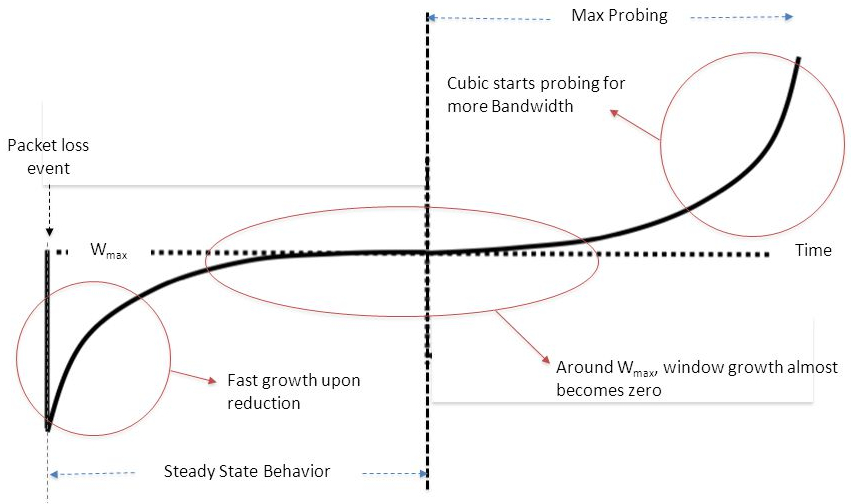
\includegraphics[scale=0.45]{TCPCubic}
  \caption{Image explaining how TCP Cubic works.}
\end{figure}

In this TCP version the congestion window (cwnd) is a cubic function of time
since the last congestion event.
The inflection point (of a cubic function) is set to the window prior to the
last congestion event.

TCP Cubic does not rely on the receipt of ACKs to increase the cwnd, it
depends only on the last congestion event. This is good, but leads to a less
RTT-unfairness.

This version of TCP is currently used in Linux OSes, thus there is the
possibility to change with another one.
